\chapter{交流系统短路电流计算}
\section{短路计算目的}
\begin{enumerate}
	\item 作为设备选型的依据。  
	\item 作为继电保护整定的依据。 
	\item 作为车辆主保护电器选择的依据。
\end{enumerate}
\section{短路电流计算分析}
最大短路电流出现的条件有两方面考虑。首先,需要考虑电力系统的远景规划,通常按照运行后5-10年的系统容量增加可能性以及系统运行方式的变化,这些变化可能导致系统参数改变,进而导致短路电流增大。一般来说,以系统的最大运行方式作为最大短路电流计算的条件,这包括所有发电机组都投入运行,变压器和并联输电线路都并网运行的情况,因为在这种情况下系统供给的短路电流最大。


另一方面,针对设计的牵引变电所或其他供电装置,其本身的主接线和运行方式也会对短路电流的数值产生显著影响。因此,在初步确定主接线和主变压器运行方式的情况下,需要选择电气设备可能处于最严重短路电流状态的短路点,作为短路电流计算点。这有助于确定在系统的最大运行方式下,通过各种电气设备和载流母线的最大短路电流。


通过分析青岛—海阳城际轨道供电图,我们可以了解到,当土寨河主变电所建成后,全线将分成8个供电分区。此外,还设有两个应急联络开关,分别位于北九水站和蓝色硅谷站。因此,在计算短路电流时,需要考虑正常运行和故障运行情况。
\section{短路电流计算}
变压器的参数计算结果如下:
$$
R_T=\frac{P_kU_{N}^{2}}{1000S_{N}^{2}}=\frac{215\times 35^2}{1000\times 31.5^2}=0.265\left( \Omega \right) 
$$
$$
X_T=\frac{U_d\%}{100}\times \frac{U_{N}^{2}}{S_N}=\frac{10.5}{100}\times \frac{35^2}{31.5}=4.083\left( \Omega \right) 
$$
\begin{figure}[h]
	\centering
	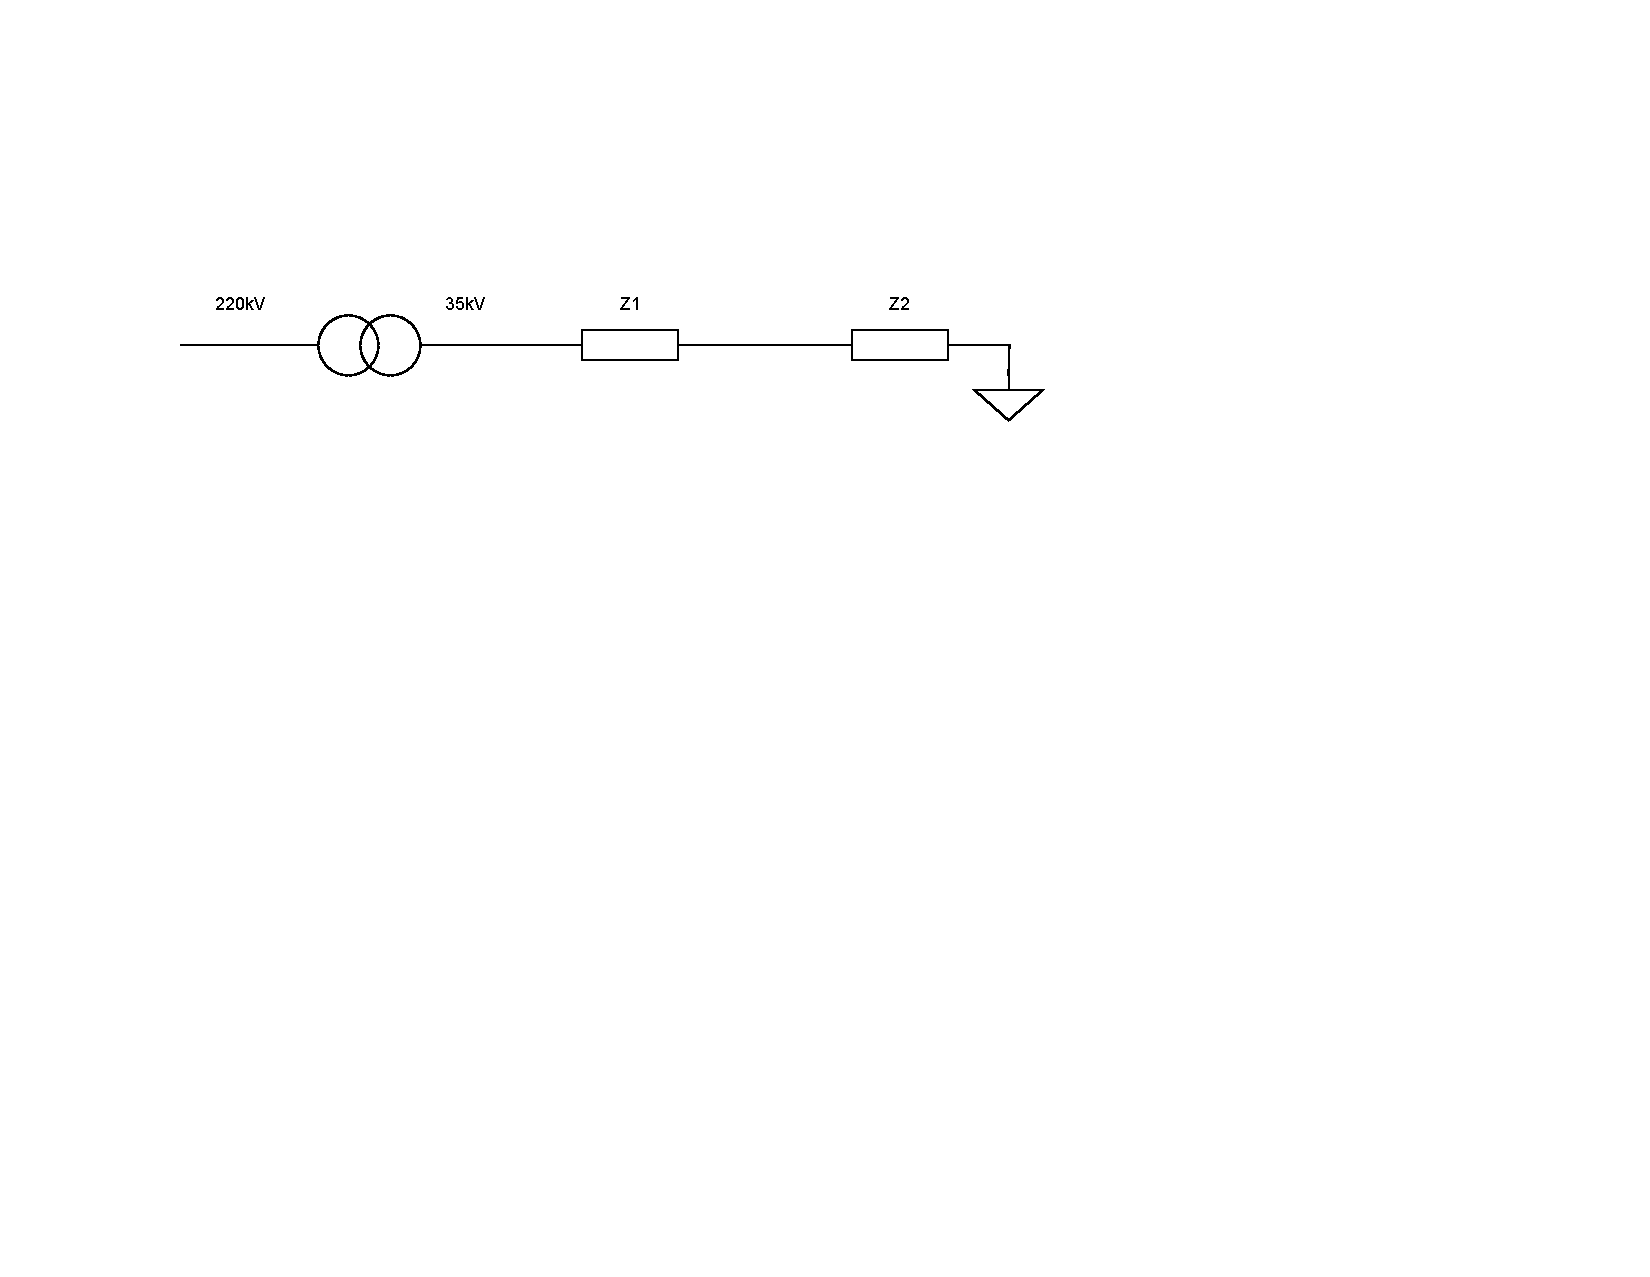
\includegraphics[width=0.9\textwidth]{电路图1.pdf}
	\caption{等效电路图}
\end{figure}
水泊站计算过程如下:
\begin{subequations}
	\begin{align}
Z_T=&R_T+jX_T=0.265+j4.08\left( \Omega \right) \label{}
\\
Z_1=&10\times \left( 0.054+j0.103 \right) =0.54+j1.03\left( \Omega \right) \label{}
\\
Z_2=&( 3.257+2.567+2.819 ) \times \left( 0.09+j0.104 \right) \notag
\\
=&0.77787+j0.898871\left( \Omega \right) \label{}
\\
Z_{\text{总}}=&Z_T+Z_1+Z_2\approx 1.58+j6\left( \Omega \right) \label{key}
\\
I=&\frac{U_k}{\sqrt{3}Z_{\text{总}}}=\frac{37.5}{\sqrt{3}\times |Z_{\text{总}}|}=\frac{37.5}{\sqrt{3}\times \sqrt{1.58^2+6^2}}=3.489\left( kA \right)\label{key}
	\end{align}
\end{subequations}
山东大学站计算结果如下:
\begin{subequations}
	\begin{align}
		Z_2=&( 8.643+2.215+1.798 ) \times \left( 0.09+j0.104 \right) \notag
		\\
		=&1.13904+j1.316224\left( \Omega \right) \label{}
		\\
		Z_{\text{总}}=&Z_T+Z_1+Z_2\approx 1.9+j6.4\left( \Omega \right) \label{key}
		\\
		I=&\frac{U_k}{\sqrt{3}Z_{\text{总}}}=\frac{37.5}{\sqrt{3}\times |Z_{\text{总}}|}=\frac{37.5}{\sqrt{3}\times \sqrt{1.9^2+6.4^2}}=3.243\left( kA \right)\label{key}
	\end{align}
\end{subequations}
\begin{figure}[h]
	\centering
	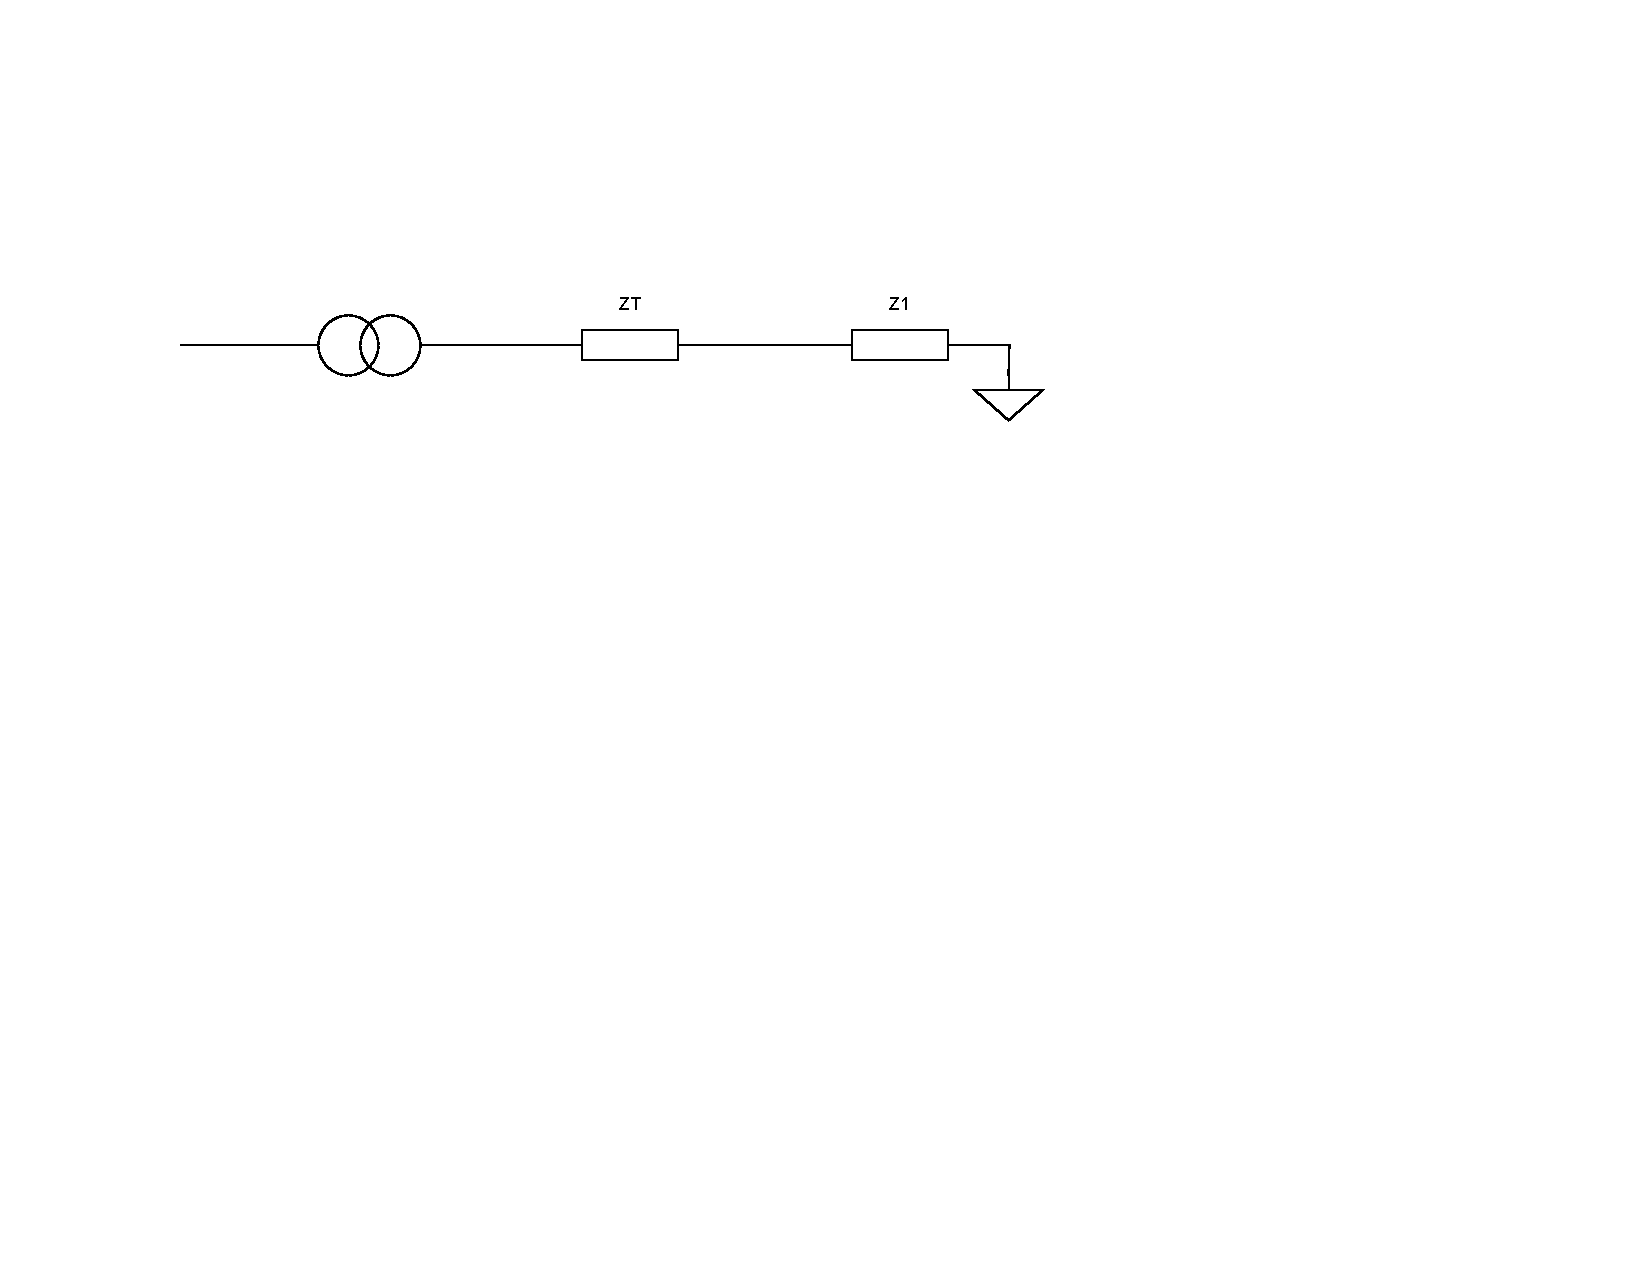
\includegraphics[width=0.9\textwidth]{电路图2.pdf}
	\caption{开闭所等效电路图}
\end{figure}
\begin{subequations}
	\begin{align}
		Z_T=&0.265+j4.08\left( \Omega \right) \label{key}
		\\
		Z_1=&0.54+j1.03\left( \Omega \right) \label{key}
		\\
		Z=&Z_T+Z_1=0.8+j5.1\left( \Omega \right) \label{key}
		\\
		I=&\frac{U_k}{\sqrt{3}Z}=\frac{37.5}{\sqrt{3}\times |Z|}=\frac{37.5}{\sqrt{3}\times \sqrt{0.8^2+5.1^2}}=4.2\left( kA \right) \label{key}		
	\end{align}
\end{subequations}
综上,在水泊站的最大短路电流最大,故在进行设备选型中采用在$3.489kA$的最大短路电流代入计算。